%\let\textcircled=\pgftextcircled
\chapter{Rotation with quaternions}
\label{chap:rotation_with_quaternions}

This chapter deals with the usage of quaternions for rotations and in general with all of the project parts related to the transformation from a local frame of reference to a laboratory one.

\section{From local to laboratory}
The program calculates the change of angular positions by integrating angular velocities, which are described in a local reference frame. This means that for calculating angular position at time $t_{i+1}$ we must take into account angular position at time $t_i$, so that it is reconstructed iteratively.\\
\begin{figure}[H]
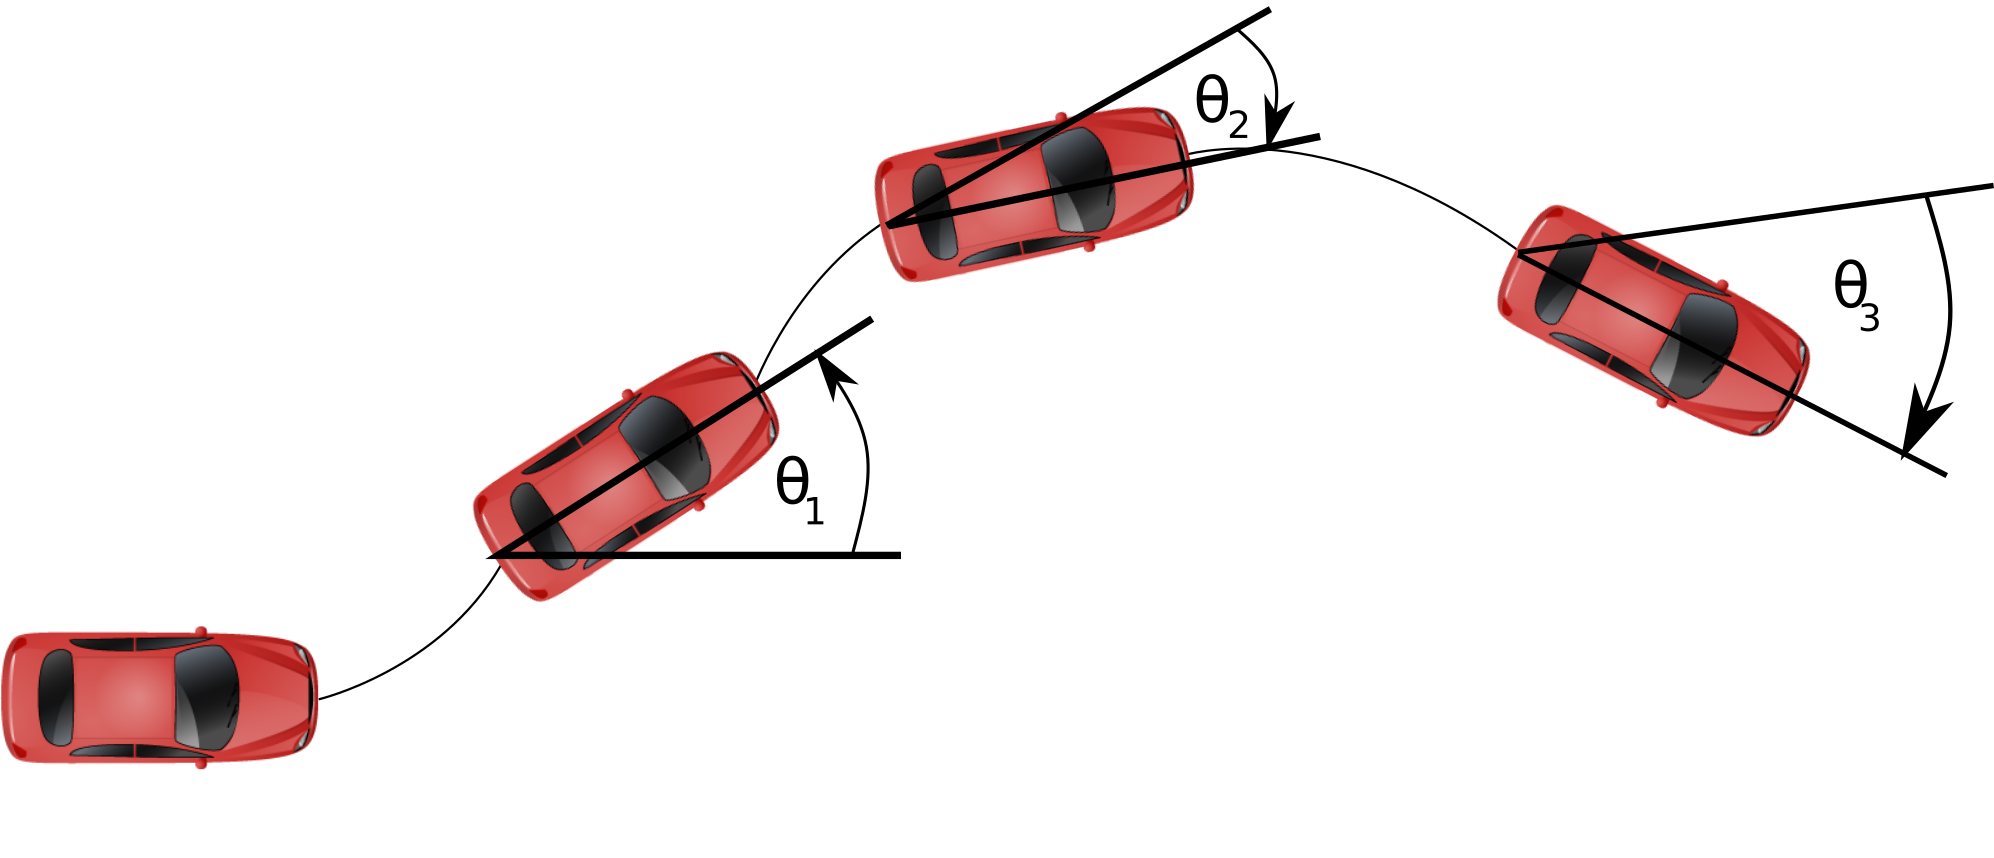
\includegraphics[width=\textwidth]{angle_composition.png}
\caption{Angle composition in vehicle motion}
\end{figure}
\justify
One of the first error I committed was to consider the rotation composition as the sum of angles on each axis. I was using the same integration routine used for linear dimensions, which performs the cumulative sum on each axis independently,  i.e. the sum of the areas. When composing multiple rotations, for example when having a rotation around vertical versor $\hat{z}$ by an angle $\theta_z$, besides adding $\theta_z$ to the vertical rotation, one must move rotation axes that belongs to the horizontal $xy$ plane. \\
So I divided the integration routine in two functions, one that returns an array of areas, the other that calls the first and then does the cumulative sum of the array of areas. I've done this also for keeping compatibility with others modules that were using the previous single function. \\
Then, once I had the angle variation vector $\langle\Delta\theta_x,\Delta\theta_y,\Delta\theta_z\rangle$ the associated quaternions can be created and multiplied together. 
Essentially, the two quaternion libraries I used in the project overload mathematical operators so compositions and rotations become more straightforward. \\
For quaternion composition, initially I was using \texttt{numpy.cumprod()} \cite{numpy-cumprod} but this function was performing multiplications in reverse order, with respect to what I needed for my application. For example, calling \texttt{cumprod()} on a vector $\langle a,b,c,d \rangle$ will result in $\langle a,ab,abc,abcd \rangle$ while I needed $\langle a,ba,cba,dcba \rangle$  \\
\\
\justify
So I wrote some custom code to make quaternion composition, using \texttt{functools.reduce()}, since it's faster than using a \texttt{for} cycle.

\begin{lstlisting}[language=Python,frame=single]
quaternions = reduce(lambda array, element: [*array, element * array[-1]], 
					quaternions, 
					[initial_quaternion])
\end{lstlisting}
The reason is that lambda use local scoped variables, that can be kept in register and cache, and that interpreter can preload next items.
%TODO explain previus code, comparison with for cycle, proof that is faster
%TODO talk about how to create a quaternion, difference in creating a quaternion representing a rotation from one that represent a vector to be rotated.
%TODO also talk about map for rotation


\section{World frame of reference}
There exists an additional frame of reference, similar to the laboratory one described before but with an additional rotation in the horizontal plane. This frame of reference has y-axis oriented towards geographical north and x-axis to east. This is critically important for mixing GNSS data that is already in this frame of reference, with integrated inertial data. \\
To find the angle between GNSS positions and east, the program finds the first position that is at least 10 meters away from the initial one, then calculates the angle of this vector. \\
Assuming that the first motion of the vehicle is in the forward, direction given the previous calculated angle, all accelerations should be rotated. \\
Instead of rotating all accelerations and angular positions, the program sets only the initial position with respect to the world frame of reference. Since the following angular positions are calculated from the first, no additional operations are needed, preventing the execution of $O(n)$ operations, i.e. the rotation of all records.